\chapter{Related Work}
\thispagestyle{plain}

\label{Chapter2}

In this section we described about other researches that are relevant to our work. They can be categorized into two major criterias; cybersecurity and event extraction. The details are as followed:


\section{Cybersecurity}
\label{CyberResearch}

	There are several researches that had been done about a decade in our Ebiquity research group. These researches can be classified into two groups; creating new ontologies for cybersecurity, and cybersecurity information extraction from structured and unstructured text. We will summarized them ordered by year and their researches’ aspects. 

\subsection{Cybersecurity Ontologies}

There are two major ontology development in the past of Ebiquity research group. The first one is IDS-Intrusion Detection System done by \cite{undercoffer2003} and \cite{undercoffer2004}. The second is UCO-Unified Cybersecurity Ontology done by \cite{syed2016uco}. \cite{undercoffer2003} started by comparing the cybersecurity standard that uses XML to define its data model with their invented ontology. Their ontology specified a model of computer attack using the DARPA Agent Markup Language+Ontology Inference Layer, a descriptive logic language. They focused on low level kernel attributes at the process, system and network levels, to serve as those taxonomic characteristics. They demonstrated use cases scenario and presented benefits of using the ontology in the intrusion detection system. Then in \cite{undercoffer2004} have produced an ontology specifying a model of computer attacks. Their ontology is based upon an analysis of over 4,000 classes of computer intrusions and their corresponding attack strategies and is categorized according to: system component targeted, means of attack, consequence of attack and location of attacker. 
System component class is comprised of; 
Network class is inclusive of the network layers of the protocol stack. 
System class includes attributes representing the operating system of the host, overall memory usage (MEM TOTAL, MEM FREE, MEM SWAP) and CPU usage (LOAD AVG).
Process class contains attributes representing particular processes that are to be monitored such as the current value of the instruction pointer, the current top of the stack, a scalar value computed from the stream of system calls, and the number of child processes.\\
 The class Consequence is comprised of several subclasses which include: 
\begin{itemize}
    \item Denial of Service is the unstable state of the system or all of the system resources may be consumed by meaningless functions.
    \item User Access is when the attacker having access to services on the target system at an unprivileged level.
    \item Root Access is when the attacker being granted privileged access to the system, consequently having complete control of the system.
    \item Probe is when the system profiles or system activities are scan and disclosed.  
\end{itemize}
The class Means of attack contained subclasses:
\begin{itemize}
    \item Input Validation Error. An input validation error exists if some malformed input is received by a hardware or software component and is not properly bounded or checked. This class is further subclassed as: (a) Buffer Overflow. (b) Boundary Condition Error. (c) Malformed Input.
    \item Logic Exploits. Logic exploits are exploited software and hardware vulnerabilities such as race conditions or undefined states that lead to performance degradation and/or system compromise. Logic exploits are further subclassed as follows: (a) Exception Condition. (b) Race Condition. (c) Serialization Error. (d) Atomicity Error.
\end{itemize}
 These classes have defined relationship as shown in Figure \ref{fig:idsontology}.

\begin{figure}
    \centering
    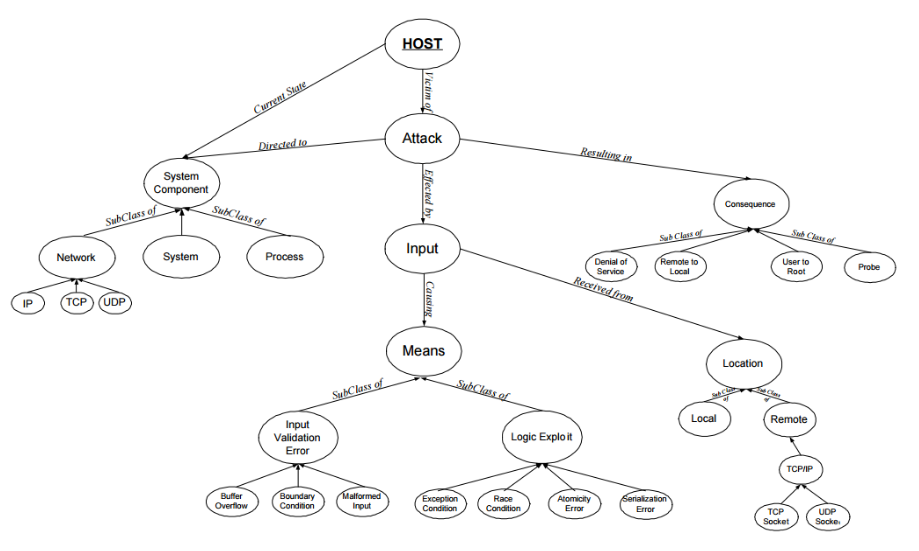
\includegraphics[width=\textwidth]{idsontology}
    \caption{Target-centric ontology}
    \label{fig:idsontology}
\end{figure}

After that, \cite{syed2016uco} invented the Unified Cybersecurity Ontology (UCO) that is intended to support information integration, information sharing and exchange and cyber situational awareness in cybersecurity system. The UCO is an extension to Intrusion Detection System ontology (IDS) (Undercoffer et al., 2004). UCO has been extended with a number of relevant cybersecurity standards, vocabularies and ontologies such as CVE, CCE, CVSS, CAPEC, CYBOX, KillChain and STUCCO. Besides, UCO also maps concepts to general world knowledge sources i.e. Linked Open Data cloud, Google’s knowledge graph, DBpedia, Yago. UCO contains important classes as following:
\begin{itemize}
    \item Means class describes various methods of executing an attack. 
    \item Consequences class describes the possible outcomes of an attack. 
    \item Attack class characterizes a cyber threat attack. 
    \item Attacker class represents identification or characterization of the adversary. 
    \item AttackPattern class are descriptions of common methods for exploiting software.  
    \item Exploit class characterizes description of an individual exploit.
    \item Exploit Target class are vulnerabilities or weaknesses in software, systems, networks or configurations.
    \item Indicator class contains patterns identifying certain observable conditions as well as contextual information about the patterns meaning, how and when it should be acted on.
\end{itemize}
Besides these classes they also design classes that uses for supporting other cybersecurity standard such as; CCE, CVE, CVSS, Weakness, Malware , Network state, OSVDB, Source, KillChain, KillChain phase.

\subsection{Cybersecurity Information Extraction}
\label{cybersecuie}
The information extracted by these researches are computer entities, concepts. The data sources are web text, NVD, vulnerabilities. Some of them applied IDS or UCO. None of them is about cyber security events. \cite{mulwad2011} developed a framework to detect and extract information about vulnerabilities and attacks from Web text. The system can process a stream of text to detect potential vulnerability descriptions and extract concepts and topics of interest as well as associated entities such as software products. They trained an SVM classifier to recognize text segments likely to contain security related information using the standard unigram bag of words vector model. They use OpenCalais to extract entities like organizations and software products. Then extract concepts related to computer security exploits by using the knowledge from Wikitology along with a computer security exploit taxonomy extracted from Wikipedia to identify vulnerabilities, threats and attacks.

\cite{more2012} presented a situation-aware intrusion detection model by collecting information from heterogeneous data source and build a semantically rich knowledge base and using reasoner to detect cyber threat. The cyber threat data are collected from several resources such as Cacti, Nagios, Wireshark, IDS/IPS modules, logs data from hardware sensors like Cisco, Web data, NVD database. These cybersecurity entities and information will be extracted by OpenCalais and mapped into the classes in the ontology in knowledge base in N3 format. These N3 triples are used by the reasoning algorithm to deduce an occurrence of threats or attacks. 

\cite{lal2013} developed a system that automatically extracts the terms from Cybersecurity blogs and security bulletins using Natural Language Processing (NLP) and text mining methods. Their named entity recognition model is trained on conditional random fields (CRFs) based on Stanford NER. There are seven types of entities; Software, Network terms, Attack (Means and Consequences), Filename, Hardware, Other technical terms, and NER modifier. Nine features are chosen to trained with vulnerability data from NVD and Microsoft and Adobe Security Bulletins. The results showed the good performance in extracting the cybersecurity entities from unstructured text.

\cite{joshi2013extracting} and \cite{joshi2013linked} published a RDF linked data representation of cybersecurity concepts  based on information from National Vulnerability Database (NVD) and developed an automatic system to recognize and extract relevant information from vulnerability descriptions that are in unstructured text format. A CRF-based system is used to identify cybersecurity-related entities, concepts and relations in text, which are then represented using custom ontologies for the cybersecurity domain and also mapped to objects in the DBpedia knowledge base. The result showed that their system provides a robust, scalable and effective model to identify terms and concepts described in the NVD dataset, gathers further information about the threat from associated repositories, extracts information from free text, models the data by aligning it to a custom ontology, and generates RDF linked data that is made available via a SPARQL endpoint. However, this framework does have a few limitations, especially in terms of cross referencing entities in the RDF graph based on the text description, and resolving identifies concepts to relevant documents on the Web.

Recently, \cite{mittal2016cybertwitter} presented a framework to analyze tweets about cybersecurity and issued threat alerts to security analysts based on the organization’s system profile. They collected tweets and extracted cybersecurity entities and concepts using (Lal et al., 2013). These cybersecurity terms and concepts are converted to RDF triples using UCO ontology (Syed et al., 2016) and then are stored in the Cybersecurity knowledge base. The alert system will use their SWRL rules to reason over these data and issue alerts based on the User system profile. UCO did provide their domain overview of cybersecurity but it does not contain any temporal properties in the ontology so they added more properties in the ontology. These additional properties are hasCounter, hasBeginTime, hasLastIntelTime, hasVulnerability, productInUSP, isCurrentlyValid. 


\section{Events}
\label{events}
This section we will describe about event ontologies and event extraction researches.
\subsection{Event Ontologies}
\label{eventontologies}
There are some research that design ontology for storing event information. Usually, each research has its own definition of event. All of them contained some different. \cite{raimond2007event} defined event as the way which cognitive agents classify arbitrary time/space regions. Their ontology has been proven useful in a wide range of context, such as talks in a conference, description of concert or chords. Their event concept is that an event may have a location, a time, agents, factors and products. These are core classes as depicted in Figure \ref{fig:eventontoYves}. \\
\begin{figure}
    \centering
    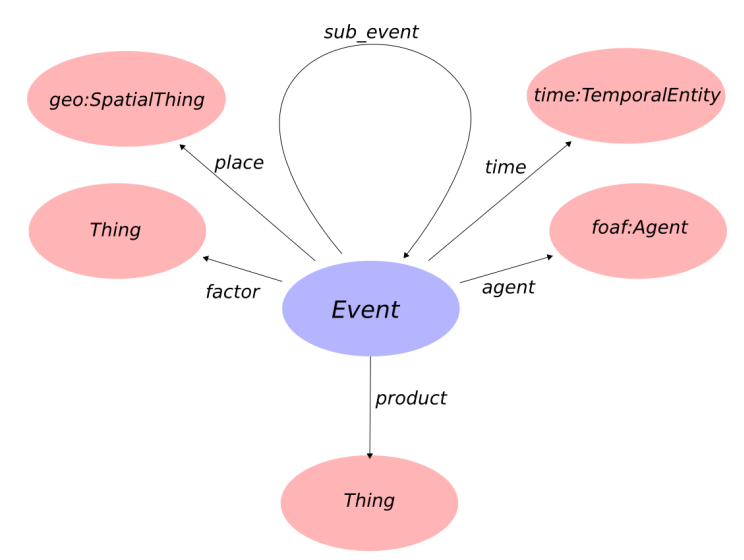
\includegraphics[width=0.6\textwidth]{eventontoYves}
    \caption{The Event Ontology by (Raimond and Abdallah 2007)}
    \label{fig:eventontoYves}
\end{figure}
\indent \cite{van2011design} designed The Simple Event model (SEM). They defined event as central elements in the representation of data from a variety of domains such as history, cultural heritage, geography and multimedia. Event-centered modeling captures the time and place aspects of a domain. In particular these aspects of viewpoints: (1) Event bounded roles, (2) time bounded validity of facts (e.g. time dependent type or role), and (3) attribution of the authoritative source of a statement. They have four core classes: sem:Event (to record what happens), sem:Actor (who or what participated in the event), sem:Place (where did it happen), sem:Time (when did it happen). Their classes and relationships are shown in Figure \ref{fig:eventontowillem}.\\
\begin{figure}
    \centering
    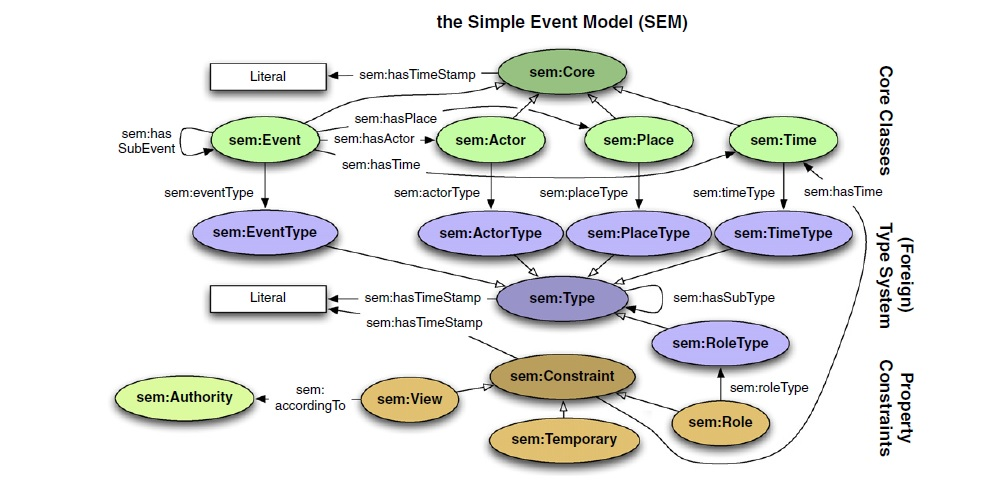
\includegraphics[width=\textwidth]{eventontowillem}
    \caption{The Event Ontology by (Van Hage et al. 2011)}
    \label{fig:eventontowillem}
\end{figure}
\subsection{Event Extraction Research}
\label{eventextractionresearch}
There are a lot of researches have been done about information extraction including event. Not only individual research has been experimenting, but also the shared task which the organizer defined the problem and graded the solution of each participant. The well known shared task that focused on event extraction problem as one of many tracks is called Text Analysis Conference or TAC. They have been provided corpus and evaluation process for event extraction for many years. We summarized the researched that participated in the TAC for 2015 and 2016 in the first subsection. After that, other individual researches also were mentioned.
\subsubsection{TAC 2015 and 2016 Event Track}
\label{tac}
Because of TAC is a shared task, they have to provided the event annotation guidelines likes the standard among all of the participants. This guidelines called Rich ERE (entities, relations, and events). In the guidelines (Linguistic Data Consortium, 2016), The taggable event is defined as \\ \\
\textit{"A taggable event is an explicit occurrence of an event with or without  participants. The goal of event annotation is to detect and characterize events  that tagged entities and argument fillers participate in, and to perform event coreference."} \\ \\
\indent Besides, events are also classified into 8 types 38 subtypes such as Life.Die, Conflict.Attack, Personnel.StartPosition. These events types/subtypes were reduced into 8 types 18 subtypes in 2016. Each event types/subtypes has definition and examples provided in the guidelines for the best understanding of the problem among participants. The evaluation metric contained four F1 measurements; (1) Span only: no attribute are considered other than span. (2) Type: consider the type attribute. (3) Realis: consider the Realis attribute and (4) All: consider all attributes. But we will focused only the second F1 “Type” because in this dissertation we will not considered “Realis” or reality of the event. We selected some of the high ranked participants’ researches and summarized them in two aspects; features, and learning algorithms. We also participated in the TAC shared task in these two years. Our own work will be described in the preliminary work section.\\
\indent (Lu Ng, 2016) participated in 2016. They got F1 scores of 46.99. They have four 1-nearest neighbor models with Jaccard to measure the distance between each pair of instances. Output is the union of event mentions and their subtypes identified in each pass. Model1 used verb triggers, used the head words of their subjects and objects as features, where the subjects and objects are extracted from dependency parse trees obtained using the Stanford CoreNLP (Manning et al., 2014). Model2 used verb triggers, and used the entity types of their subjects and objects as features. Model3 used the WordNet synset ids of the trigger and its hypernym as features. Model 4 used the unigrams in the sentence in which the trigger appears as features.\\
\indent (Liu et al., 2016) participated in 2016. They got F1 scores of 44.61. They used a discriminatively conditional random fields (CRF) model to detect mention span and event. The CRF model is trained with the structured perceptron. Features consisted of the target word itself and the direct dependent words of the target, coarse part-of-speech (2-character), lemma, lemma+pos and named entity tag of words in the 2-word window of the target (both side), The combination of previous and next word’s part-of-speech and lemma with the target word’s part-of-speech and lemma, Brown clusters, WordNet Synonym and derivative forms of the trigger, whether surrounding words match some selected WordNet senses, these senses are ”Leader”, ”Worker”, ”Body Part”, ”Monetary System”, ”Possession”, ”Government”, ”Crime” and ”Pathological State”, closest named entity type, dependency features, including lemma, dependency type and part-of-speech of the child dependencies and head dependencies, Semantic role related features includes the frame name and the argument role, named entity tag,argument headword lemma and WordNet sense.\\
\indent (Zeng et al., 2016) participated in 2016. They got F1 scores of 44.35. They have two methods; feature-based model, neural network model, and ensemble their outputs at last by majority voting. Feature-based model consists of two steps; trigger identification, trigger classification. For trigger identification, two traditional classifiers, a Max Entropy model and a Conditional Random Field (CRF) model had been used with features. Features are word, part-of-speech tag, lemma, and stem respectively, Wordnet synset indicates the WordNet synset that word belongs to. For trigger classification was built with a Max Entropy model to perform the type classification task. Features used in this model consist of  word, stem, Wordnet synset, nearest entity. For neural network model, Bidirectional Long Short Term Memory had been introduced with a CNN layer. For each event type, a neural network model that labels each sentence in the BIO scheme. Specifically, a word is labeled as B if it is he beginning of a trigger of type ,or I if it is inside a trigger of type, or O otherwise. The 100-dimension word embeddings are pretrained on the training set, and fine-tuned during training. In LSTM, the state size is 100. As for CNN, the sliding window size is 7 (3 words to the left and to the right of a center word),and the kernel sizes are set from 2 to 7 to capture context information of various granularities.\\
\indent \cite{reimers2015event} participated in 2015. They go F1 scores of 55.56. They trained a deep feed forward network. Features consist of the lemma of each word, the part-of-speech tag and, if present,  the capitalization, the subject and object linked to the token based on the parse tree, the initial and final 2 to 6 characters of the token, the word-shape3 given by wordShapeChris2 from Stanford CoreNLP, and a feature to indicate that tokens are inside quotes. They used a context window size of 3. For the lookup of the lemmas, they used the pre-trained word embeddings by Levy and Goldberg (2014) on the English Wikipedia using dependency links as context. They also used the pre-trained word embeddings by Mikolov et al. (2013) on the Google News dataset. The embeddings by Levy,et.al. capture syntactic similarity well, while the vectors trained on the Google News dataset capture semantic similarity well. The combination of both embeddings allows the neural network to choose the more suitable embeddings for the task. They also allowed the embeddings to be updated during training. These networks were trained only on event mentions, ignoring all other non-event tokens. \\
\indent \cite{hong2015rpi} participated in 2015. They got F1 scores of 58.41. They used a Maximum Entropy model (MaxEnt) to predict the event type, based on linguistic features; neighbor grams and part-of-speech tag, lemma, synonyms and case of the target token, Brown clusters, dependent and governor words, whether the target token is a non referential pronoun, whether the target is a modifier of job title, types of entities within the text window of size 3 if have, types of dependent and governor entity of the target token, argmax event type of the target token in training data. They used this MaxEnt model as a baseline, and also introduced Topic modelling to improve the performance.\\
\indent \cite{monahan2015populating} participated in 2015. They got F1 scores of 57.18. The system is a pipeline consisting of event discovery, prior probability estimation, contextual probability, and event extraction. The event discovery module used for searching in text find any words that are possibly trigger. It tried to match candidate triggers against lexicon using the exact form found in the lexicon sources, or the porter-stemmed form, or any derived form. Then compute a prior probability with each lexical item ( $P(Eventtype|Lexicon)$) , after that a contextual system considered whether the predicted event type is correct. Finally, the logistic regression model was trained to make the final determination to accept or reject each candidate trigger. 
\subsubsection{Individual Research}
\label{eventresearch}
	Besides those shared task system, event extraction also been researched individually among researchers. We selected some of researches that has been cited by other researches in the event extraction area. The researches were summarized only their goal, method and features.

\cite{ji2008refining} introduced consistency at several levels to help in event extraction process. These consistencies are : consistency of word sense across different instances of the same word in related documents, and consistency of arguments and roles across different mentions of the same or related events. They mentioned two motivations; one trigger sense per cluster means: if we can determine the sense (event type) of a word in the related documents, this will allow us to infer its sense in the test document. find trigger’s sense from related document (not in training corpus), and one role per cluster means: each entity plays the same argument role, or no role, for events with the same type in a collection of related document. In summary, they used their baseline system to extract triggers and arguments from the test document, and then use these triggers and arguments to form query to select related document to find trigger sense or argument additional information from these related document, and then compute some confident values and validate with their rules to help verify the accuracy of the extracted triggers and arguments.

\cite{liao2010using} proposed event extraction system that identified event triggers and event arguments, which is a two-pass system; sentence-level and document-level. There design based on statistical facts; there is a strong trigger consistency within the document, there are also strong correlations among event types in a document, if an entity appears as an argument of multiple events of the same type in a single document, it is assigned the same role each time. Two Maximum Entropy (MaxEnt) classifiers – a document-level trigger and argument classifier were built. The document-level trigger classifier features consist of the base form of the word, event type, binary indicator of whether this event type is present elsewhere in the document. The document-level role classifier feature are the event type that is trying to assign an argument/role to, one of the other event types, the role of this entity with respect to the other event type elsewhere in the document, or null if this entity is not an argument of that type of event. Experiments showed that document-level information can improve the performance of a sentence-level baseline event extraction system. The experiments proved that the perceptron with local features outperforms the staged baseline and the global features further improve the performance significantly, surpassing the current state-of-the-art by a large margin. 

\cite{li2013joint} presented a framework for sentence level event extraction, which predicts triggers and their arguments jointly. They used structured perceptron with inexact search to jointly extract triggers and arguments that co-occur in the same sentence. Features were categorized into local and global feature. Local features are only related to predictions on individual trigger or argument whereas global features involved longer range of the output structure. Examples of local features are unigram/bigram of the target word, part-of-speech tag of the target word. Global features are the relations between triggers or arguments such as bigram of trigger types in the same sentence, dependency path between two triggers, features about two arguments of an event mention which are overlapping.

